\documentclass[a4paper,12pt]{report}
\usepackage[latin1]{inputenc}
\usepackage{amsmath}
\usepackage{amsmath,bm}
\usepackage{amsthm}
\usepackage{mathtools}
\usepackage{amsfonts}
\usepackage{amssymb}
\usepackage{graphicx}
\usepackage{array}
\usepackage{booktabs}
\usepackage{hyperref}
\usepackage{multicol}
\usepackage[margin=0.5in]{geometry}
\usepackage{karnaugh-map}
\usepackage[framemethod=tikz]{mdframed}
\begin{document}
\raggedright{
\includegraphics[scale=0.07]{logo.jpg}}\hspace{12.425cm}\raggedleft FWC22025\vspace{2mm}
\\
\centering\Large\textbf{ASSIGNMENT-MATRICES}\vspace{5mm}


\begin{multicols}{2}
\centering \large\textsc{C}\footnotesize\textsc{ONTENTS}\vspace{5mm}
\\
\raggedright\large\textbf{1\hspace{1cm}Problem}\hspace{5.18cm}1\vspace{5mm}\\
\raggedright\large\textbf{2\hspace{1cm}Solution}\hspace{5.25cm}1\vspace{5mm}\\
\raggedright\large\textbf{3\hspace{1cm}Construction}\hspace{4.1cm}2\vspace{5mm}\\


\centering \large\textsc{1  P}\footnotesize\textsc{ROBLEM}\vspace{5mm}\\
\hspace{1cm}\large If E,F,G and H are respectively the mid-points of the sides of a parallelogram \\ \raggedright ABCD, show that \\
\centering{ar(EFGH) =$\frac{1}{2}$ ar(ABCD)}\vspace{5mm} 


\centering \large\textsc{2  S}\footnotesize\textsc{OLUTION}\vspace{5mm}\\
\raggedright\large{1. Construct a parallelogram with vertices A,B,C and D.}\\
\raggedright\large{2. Point mid-points E,F,G and H on sides AB,BC,CD and DA.}\vspace{5mm}\\
\hspace{2cm}\normalsize\textbf{E = $\frac{\normalsize\textbf {A+B}}{\normalsize\textbf 2}$}\vspace{2mm}\\
\hspace{2cm}\normalsize\textbf{F = $\frac{\normalsize\textbf{B+C}}{\normalsize\textbf 2}$}\vspace{2mm}\\
\hspace{2cm}\normalsize\textbf{G = $\frac{\normalsize\textbf {C+D}}{\normalsize\textbf 2}$}\vspace{2mm}\\
\hspace{2cm}\normalsize\textbf{H = $\frac{\normalsize\textbf {D+A}}{\normalsize\textbf 2}$}\vspace{5mm}\\
\raggedright\large{3. By joining the midpoints of adjacent sides of parallelogram ABCD, another parallelogram EFGH is formed.}\\
\raggedright\large{4. Join EG.}\\
\raggedright\large{5. Now draw a perpendicular from point H to line EG and mark as point P,similarly from point F to line EG and mark as point Q.}\vspace{5mm}\\


\raggedright\large{Then,}\vspace{2mm}\\
\centering\normalsize\textbf{ar(AEGD) = $ \| \normalsize\textbf{(E-G)(H-P)} \| $} -- (1)\vspace{2mm}\\
\centering\normalsize\textbf{ar(EHG) = $\frac{\normalsize\textbf 1}{\normalsize\textbf 2}$ $ \| \normalsize\textbf{(E-G)(H-P)} \| $} -- (2)\vspace{2mm}\\

\raggedright\large{Similarly,}\vspace{2mm}\\
\centering\normalsize\textbf{ar(BEGC) = $ \| \normalsize\textbf{(E-G)(F-Q)} \| $} -- (3)\vspace{2mm}\\
\centering\normalsize\textbf{ar(EFG) = $\frac{\normalsize\textbf 1}{\normalsize\textbf 2}$ $ \| \normalsize\textbf{(E-G)(F-Q)} \| $} -- (4)\vspace{5mm}\\

\raggedright\large{From (1) and (2),}\vspace{2mm}\\
\centering\normalsize\textbf{ar(EHG) =  $\frac{\normalsize\textbf 1}{\normalsize\textbf 2}$ ar(AEGD)} --(5)\vspace{2mm}\\

\raggedright\large{From (3) and (4),}\vspace{2mm}\\
\centering\normalsize\textbf{ar(EFG) =  $\frac{\normalsize\textbf 1}{\normalsize\textbf 2}$ ar(BEGC)} --(6)\vspace{10mm}\\

\raggedright\large{From (5) and (6),}\vspace{2mm}\\
\raggedright\normalsize\textbf{ar(EHG)+ar(EFG) = \\ \hspace{3.5cm}{$\frac{\normalsize\textbf 1}{\normalsize\textbf 2}$ ar(AEGD)+$\frac{\normalsize\textbf 1}{\normalsize\textbf 2}$ ar(BEGC)}}\vspace{2mm}\\
\raggedright\large{Hence,}\vspace{2mm}\\
\centering\normalsize\textbf{ar(EFGH) = $\frac{\normalsize\textbf 1}{\normalsize\textbf 2}$ ar(ABCD)}\vspace{5mm}\\


\centering{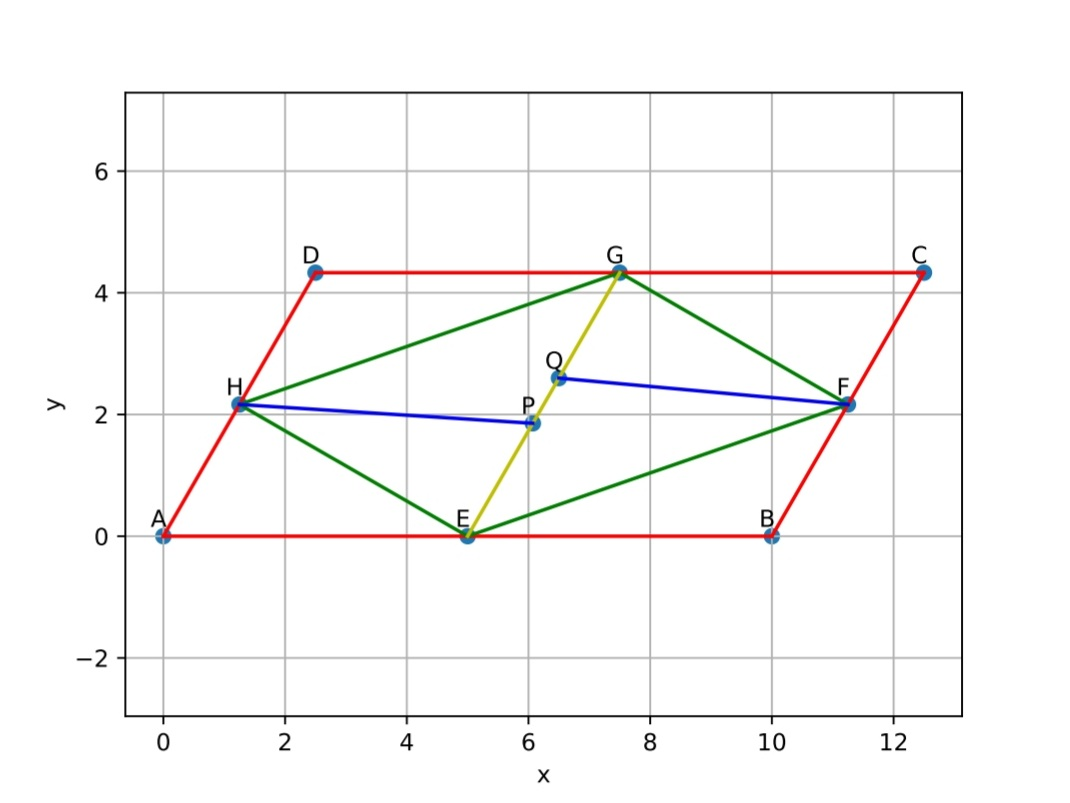
\includegraphics[scale=0.35]{main.jpg}}\vspace{2mm}\\
\centering\normalsize{Figure}\vspace{5mm}\\


\centering \large\textsc{3  C}\footnotesize\textsc{ONSTRUCTION}\vspace{5mm}\\
\raggedright\large{The parallelogram is constructed with m=10 and n=5,} 
\begin{center}
    \label{tab:truthtable}
    \setlength{\arrayrulewidth}{0.2mm}
\setlength{\tabcolsep}{5pt}
\renewcommand{\arraystretch}{2}
    \begin{tabular}{|c|c|c|}
    \hline % <-- Alignments: 1st column left, 2nd middle and 3rd right, with vertical lines in between
      \large\textbf{Symbol} & \large\textbf{Co-ordinates} & \large\textbf{Description}\\
      \hline
	\large m & 10 & \large AB \\
	\large n & 5 & \large AD\\
	\large A &  $\ \begin{pmatrix} 0\\0 \end{pmatrix}$  & \large point vector A\\
	\large B &  $\ \begin{pmatrix} m\\0 \end{pmatrix}$ & \large point vector B\\
	\large D &  $\ \begin{pmatrix} 0\\n \end{pmatrix}$ & \large point vector D\\ 
        \large C & \large B+D & \large point vector C\\ 
      \hline
   \end{tabular}
 \end{center}\vspace{5mm} 


\raggedright\large{The figure above is generated using python code provided in the below source code link.}\vspace{2mm}\\
\begin{mdframed}
\raggedright\large{https://github.com/madind5668 \\ /FWC/blob/main/assigment-4/codes/main.py}
\end{mdframed}


\end{multicols}
\end{document}